A figura mostra uma pra�a circular que cont�m um chafariz em seu centro e, em seu entorno, um passeio. Os c�rculos que definem a pra�a e o chafariz s�o conc�ntricos. 

\begin{figure}[h]
\centering
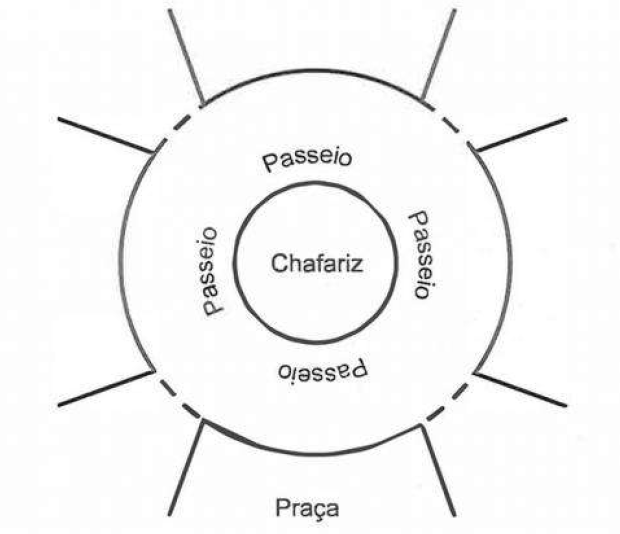
\includegraphics[width=8cm]{../figuras/q170(1)-2018.png}
\end{figure}

O passeio ter� seu piso revestido com ladrilhos. Sem condi��es de calcular os raios, pois o chafariz est� cheio, um engenheiro fez a seguinte medi��o: esticou uma trena tangente ao chafariz, medindo a dist�ncia entre dois pontos A e 8, conforme a figura. Com isso, obteve a medida do segmento de reta AB: 16 m. 


\begin{figure}[h]
\centering
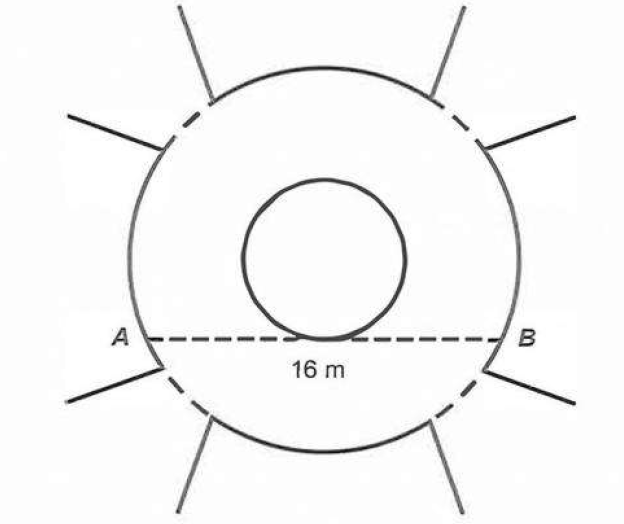
\includegraphics[width=8cm]{../figuras/q170(2)-2018.png}
\end{figure}

Dispondo apenas dessa medida, o engenheiro calculou corretamente a medida da �rea do passeio, em metro quadrado. 
A medida encontrada pelo engenheiro foi:
\newline
\\
$a)4\pi\quad b)8\pi\quad c)48\pi\quad d)64\pi\quad e)192\pi$
